
\begin{frame}{Специальная часть}{Задача компенсаторного слежения}
    \center{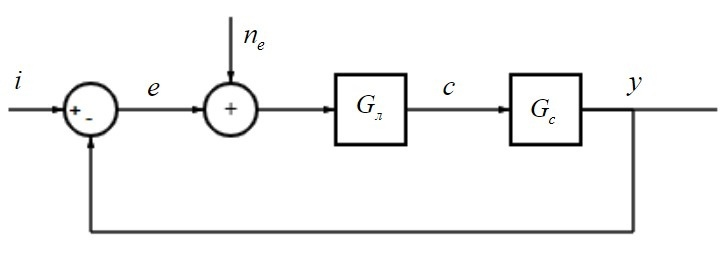
\includegraphics[width=11cm, height = 6cm]{../Оглавление/Part3/figures/СамолётЛётчик.png}}
\end{frame}
\begin{frame}{Специальная часть}{Линеаризованная модель объкта исследований}
    \begin{equation} \begin{aligned} \dot{x} = Ax+Bu \\ 
    y = Cx + Du \end{aligned} \end{equation}
$$x = \begin{bmatrix}
        V_x\\ 
        V_y\\ 
        \omega_z\\ 
        \vartheta
    \end{bmatrix},
u = \delta_\text{э}$$
   $ A = \begin{bmatrix}
        -0.0110 & 0.0433 & 1.7295 & -7.1876\\ 
        -0.0691 & -0.6975 & -7.0678 & -54.8976\\ 
        0.00011 & 0.00116 & -0.35407 & 0.0911\\ 
        0 & 0 & 1 & 0
    \end{bmatrix} ,$  
        $B = \begin{bmatrix}
        -0.4412\\ 
        -12.388\\ 
        -0.58446 \\ 
        0
    \end{bmatrix}$  
\end{frame}


 
% \begin{frame}{Специальная часть}{Собственная робастность системы}
%     \begin{block}{Коэффициенты}
%     % $m_\vartheta = 0.0911$ \\
%     % $m_{V_x} = 0.00011$ \\ 
%     % $m_{V_y} = 0.0016$ \\ 
%     % $m_{\omega_z} = -0.35407$ \\ 
%     % $m_{\delta_\text{э}} = -0.58446$ \\ 
%         Пусть система дифференциальных уравнений линеаризованной динамической системы в продольном канале управления 
%         имеет вид (2), а необходимо привести к виду (3)
%         \begin{equation}
%             \label{ESS}
%             E \dot{x} = A'x + B'u
%         \end{equation}
%         $$E^{-1}E \dot{x}= E^{-1}A'x + E^{-1}B'u$$
%         $$E^{-1}A' = A$$
%         $$E^{-1}B' = B$$
%         \begin{equation}
%             \label{SS}
%             \dot{x} = Ax+Bu
%         \end{equation}
%     \end{block}
% \end{frame}

\begin{frame}{Специальная часть}{Собственная робастность системы}
    \begin{minipage}[c]{0.45\textwidth}
        \begin{center}
        $f_1 = \dot{\omega}_z - m_{\delta_\text{э}}\delta_\text{э}$
        \end{center}
    \end{minipage}
    \begin{minipage}[c]{0.45\textwidth}
        \begin{center}
        $G_c = \frac{K}{p+K} = \frac{1}{Tp+1}$
        \end{center}
    \end{minipage}
    \begin{block}{Схема}
        \center{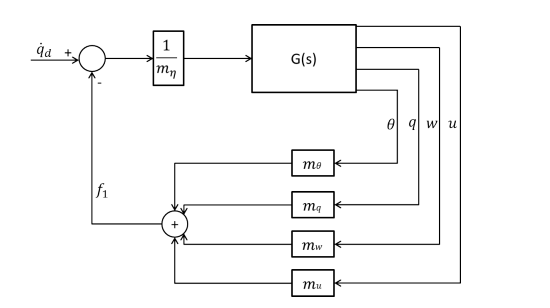
\includegraphics[width=9cm, height = 5cm]{../Оглавление/Part3/figures/Неполная схема СПС.png}}
        % %LaTeX with PSTricks extensions
%%Creator: Inkscape 1.1.2 (b8e25be833, 2022-02-05)
%%Please note this file requires PSTricks extensions
\psset{xunit=.5pt,yunit=.5pt,runit=.5pt}
\begin{pspicture}(428,147)
{
\newrgbcolor{curcolor}{0 0 0}
\pscustom[linestyle=none,fillstyle=solid,fillcolor=curcolor]
{
\newpath
\moveto(367.03192139,100.65615463)
\curveto(367.21453857,100.3446312)(367.34075928,100.05190659)(367.4105835,99.7779808)
\curveto(367.48040771,99.50942612)(367.55023193,98.97768784)(367.62005615,98.18276596)
\lineto(367.97454834,94.21889877)
\curveto(368.29681396,94.60561752)(368.76409912,95.21792221)(369.37640381,96.05581284)
\curveto(369.67181396,96.46401596)(370.03704834,97.01992416)(370.47210693,97.72353745)
\curveto(370.73529053,98.15322495)(370.89642334,98.4540062)(370.95550537,98.6258812)
\curveto(370.98773193,98.7118187)(371.00384521,98.80044174)(371.00384521,98.89175034)
\curveto(371.00384521,98.95083237)(370.98504639,98.99917221)(370.94744873,99.03676987)
\curveto(370.90985107,99.07436752)(370.81048584,99.11733627)(370.64935303,99.16567612)
\curveto(370.49359131,99.21938705)(370.36199951,99.3133812)(370.25457764,99.44765854)
\curveto(370.15252686,99.58730698)(370.10150146,99.74575424)(370.10150146,99.92300034)
\curveto(370.10150146,100.14321518)(370.16595459,100.32046127)(370.29486084,100.45473862)
\curveto(370.42376709,100.58901596)(370.5848999,100.65615463)(370.77825928,100.65615463)
\curveto(371.0145874,100.65615463)(371.21600342,100.5567894)(371.38250732,100.35805893)
\curveto(371.54901123,100.16469955)(371.63226318,99.89614487)(371.63226318,99.55239487)
\curveto(371.63226318,99.12807846)(371.48724365,98.64199448)(371.19720459,98.09414291)
\curveto(370.90716553,97.55166245)(370.34857178,96.71645737)(369.52142334,95.58852768)
\curveto(368.6942749,94.46059799)(367.69256592,93.23061752)(366.51629639,91.89858627)
\curveto(365.70526123,90.98012924)(365.10369873,90.40273666)(364.71160889,90.16640854)
\curveto(364.31951904,89.92470932)(363.98382568,89.80385971)(363.70452881,89.80385971)
\curveto(363.5380249,89.80385971)(363.39300537,89.86831284)(363.26947021,89.99721909)
\curveto(363.14056396,90.12075424)(363.07611084,90.26577377)(363.07611084,90.43227768)
\curveto(363.07611084,90.64175034)(363.16473389,90.83242416)(363.34197998,91.00429916)
\curveto(363.51385498,91.17617416)(363.70184326,91.26211166)(363.90594482,91.26211166)
\curveto(364.0133667,91.26211166)(364.10198975,91.23794174)(364.17181396,91.1896019)
\curveto(364.21478271,91.16274643)(364.26312256,91.08755112)(364.3168335,90.96401596)
\curveto(364.36517334,90.83510971)(364.41082764,90.74917221)(364.45379639,90.70620346)
\curveto(364.48065186,90.67934799)(364.51287842,90.66592026)(364.55047607,90.66592026)
\curveto(364.58270264,90.66592026)(364.63909912,90.69277573)(364.71966553,90.74648666)
\curveto(365.01507568,90.92910385)(365.35882568,91.21914291)(365.75091553,91.61660385)
\curveto(366.26654053,92.14297104)(366.64788818,92.57265854)(366.8949585,92.90566635)
\lineto(366.44378662,98.01357651)
\curveto(366.36859131,98.85683823)(366.25579834,99.36977768)(366.10540771,99.55239487)
\curveto(365.95501709,99.73501205)(365.70257568,99.82632065)(365.3480835,99.82632065)
\curveto(365.23529053,99.82632065)(365.03387451,99.81020737)(364.74383545,99.7779808)
\lineto(364.67132568,100.07607651)
\closepath
}
}
{
\newrgbcolor{curcolor}{0 0 0}
\pscustom[linestyle=none,fillstyle=solid,fillcolor=curcolor]
{
\newpath
\moveto(91.06137085,92.59087753)
\curveto(91.02377319,92.32232285)(91.00497437,92.09942245)(91.00497437,91.92217636)
\curveto(91.00497437,91.44414902)(91.17416382,91.03594589)(91.51254272,90.69756699)
\curveto(91.85092163,90.36455917)(92.2618103,90.19805527)(92.74520874,90.19805527)
\curveto(93.13192749,90.19805527)(93.50253296,90.27593613)(93.85702515,90.43169785)
\curveto(94.21688843,90.59283066)(94.74862671,90.9446373)(95.45223999,91.48711777)
\lineto(95.62142944,91.25347519)
\curveto(94.34848022,89.99126816)(93.13461304,89.36016464)(91.97982788,89.36016464)
\curveto(91.19564819,89.36016464)(90.60482788,89.60723495)(90.20736694,90.10137558)
\curveto(89.80990601,90.5955162)(89.61117554,91.14068222)(89.61117554,91.73687363)
\curveto(89.61117554,92.5371666)(89.85824585,93.35625839)(90.35238647,94.19414902)
\curveto(90.8465271,95.03203964)(91.46688843,95.68194199)(92.21347046,96.14385605)
\curveto(92.96005249,96.6111412)(93.7281189,96.84478378)(94.51766968,96.84478378)
\curveto(95.08700562,96.84478378)(95.50863647,96.72930527)(95.78256226,96.49834824)
\curveto(96.05648804,96.2673912)(96.19345093,95.99346542)(96.19345093,95.67657089)
\curveto(96.19345093,95.23077011)(96.01620483,94.80376816)(95.66171265,94.39556503)
\curveto(95.19442749,93.86382675)(94.50692749,93.43413925)(93.59921265,93.10650253)
\curveto(92.99765015,92.88628769)(92.15170288,92.71441269)(91.06137085,92.59087753)
\closepath
\moveto(91.11776733,92.98565292)
\curveto(91.91268921,93.07696152)(92.55990601,93.23272324)(93.05941772,93.45293808)
\curveto(93.72006226,93.74834824)(94.21420288,94.10015488)(94.5418396,94.508358)
\curveto(94.87484741,94.92193222)(95.04135132,95.31402206)(95.04135132,95.68462753)
\curveto(95.04135132,95.91021347)(94.96884155,96.09283066)(94.82382202,96.2324791)
\curveto(94.68417358,96.37212753)(94.48275757,96.44195175)(94.21957397,96.44195175)
\curveto(93.67172241,96.44195175)(93.08895874,96.14922714)(92.47128296,95.56377792)
\curveto(91.85897827,94.9836998)(91.4078064,94.1243248)(91.11776733,92.98565292)
\closepath
}
}
{
\newrgbcolor{curcolor}{0 0 0}
\pscustom[linestyle=none,fillstyle=solid,fillcolor=curcolor]
{
\newpath
\moveto(264.32119751,92.0190506)
\curveto(263.76260376,91.34766388)(263.19863892,90.85352325)(262.62930298,90.53662872)
\curveto(262.05996704,90.22510529)(261.45840454,90.06934357)(260.82461548,90.06934357)
\curveto(260.06192017,90.06934357)(259.46572876,90.28418732)(259.03604126,90.71387482)
\curveto(258.61172485,91.14356232)(258.39956665,91.7209549)(258.39956665,92.44605255)
\curveto(258.39956665,93.2678299)(258.62783813,94.0761795)(259.0843811,94.87110138)
\curveto(259.54629517,95.66602325)(260.16397095,96.3105545)(260.93740845,96.80469513)
\curveto(261.71621704,97.30420685)(262.47891235,97.55396271)(263.22549438,97.55396271)
\curveto(263.8109436,97.55396271)(264.24868774,97.43042755)(264.53872681,97.18335724)
\curveto(264.82876587,96.94165802)(264.9737854,96.64356232)(264.9737854,96.28907013)
\curveto(264.9737854,95.95606232)(264.87173462,95.67139435)(264.66763306,95.43506622)
\curveto(264.51724243,95.25244904)(264.3319397,95.16114044)(264.11172485,95.16114044)
\curveto(263.94522095,95.16114044)(263.80557251,95.21485138)(263.69277954,95.32227325)
\curveto(263.58535767,95.42969513)(263.53164673,95.56397247)(263.53164673,95.72510529)
\curveto(263.53164673,95.82715607)(263.55044556,95.92115021)(263.58804321,96.00708771)
\curveto(263.63101196,96.09302521)(263.71426392,96.19507599)(263.83779907,96.31324005)
\curveto(263.96670532,96.43677521)(264.04458618,96.52539825)(264.07144165,96.57910919)
\curveto(264.09829712,96.63282013)(264.11172485,96.68921661)(264.11172485,96.74829865)
\curveto(264.11172485,96.86109161)(264.06069946,96.95508575)(263.95864868,97.03028107)
\curveto(263.80288696,97.13770294)(263.58267212,97.19141388)(263.29800415,97.19141388)
\curveto(262.77163696,97.19141388)(262.25064087,97.00611115)(261.73501587,96.63550568)
\curveto(261.21939087,96.26490021)(260.77896118,95.73853302)(260.41372681,95.05640411)
\curveto(259.97329712,94.22925568)(259.75308228,93.40210724)(259.75308228,92.5749588)
\curveto(259.75308228,92.02710724)(259.90884399,91.59204865)(260.22036743,91.26978302)
\curveto(260.53189087,90.95288849)(260.95620728,90.79444122)(261.49331665,90.79444122)
\curveto(261.90689087,90.79444122)(262.31509399,90.896492)(262.71792603,91.10059357)
\curveto(263.12612915,91.31006622)(263.58267212,91.68604279)(264.08755493,92.22852325)
\closepath
}
}
{
\newrgbcolor{curcolor}{0 0 0}
\pscustom[linestyle=none,fillstyle=solid,fillcolor=curcolor]
{
\newpath
\moveto(16.68956184,104.11745071)
\curveto(16.91514778,104.11745071)(17.10582161,104.03956985)(17.26158333,103.88380814)
\curveto(17.41734505,103.72804642)(17.49522591,103.53737259)(17.49522591,103.31178665)
\curveto(17.49522591,103.09157181)(17.4146595,102.90089798)(17.25352669,102.73976517)
\curveto(17.09776497,102.58400345)(16.90977669,102.50612259)(16.68956184,102.50612259)
\curveto(16.469347,102.50612259)(16.27867317,102.58400345)(16.11754036,102.73976517)
\curveto(15.96177864,102.90089798)(15.88389778,103.09157181)(15.88389778,103.31178665)
\curveto(15.88389778,103.53737259)(15.96177864,103.72804642)(16.11754036,103.88380814)
\curveto(16.27330208,104.03956985)(16.46397591,104.11745071)(16.68956184,104.11745071)
\closepath
\moveto(16.79429817,100.91896439)
\lineto(15.19908333,95.27125931)
\curveto(15.09166145,94.88991165)(15.03795052,94.66164017)(15.03795052,94.58644485)
\curveto(15.03795052,94.50050735)(15.06212044,94.43068314)(15.11046028,94.3769722)
\curveto(15.16417122,94.32326126)(15.2259388,94.29640579)(15.29576302,94.29640579)
\curveto(15.37632942,94.29640579)(15.47300911,94.33937454)(15.58580208,94.42531204)
\curveto(15.89195442,94.66701126)(16.20079231,95.01076126)(16.51231575,95.45656204)
\lineto(16.79429817,95.27125931)
\curveto(16.4290638,94.71266556)(15.9993763,94.24269485)(15.50523567,93.8613472)
\curveto(15.1400013,93.57667923)(14.7908802,93.43434525)(14.45787239,93.43434525)
\curveto(14.23765755,93.43434525)(14.05772591,93.49879837)(13.91807747,93.62770462)
\curveto(13.77842903,93.76198196)(13.70860481,93.92848587)(13.70860481,94.12721634)
\curveto(13.70860481,94.32594681)(13.77574348,94.65626907)(13.91002083,95.11818314)
\lineto(14.95738411,98.72755814)
\curveto(15.12925911,99.31837845)(15.21519661,99.68898392)(15.21519661,99.83937454)
\curveto(15.21519661,99.9575386)(15.17222786,100.05421829)(15.08629036,100.1294136)
\curveto(15.00572395,100.20460892)(14.89293098,100.24220657)(14.74791145,100.24220657)
\curveto(14.62974739,100.24220657)(14.38536263,100.21266556)(14.01475716,100.15358353)
\lineto(14.01475716,100.46779251)
\closepath
}
}
{
\newrgbcolor{curcolor}{0 0 0}
\pscustom[linestyle=none,fillstyle=solid,fillcolor=curcolor]
{
\newpath
\moveto(153.17984009,117.63223839)
\curveto(153.15805054,117.47659874)(153.14715576,117.34741783)(153.14715576,117.24469566)
\curveto(153.14715576,116.96765709)(153.24520874,116.73108482)(153.4413147,116.53497887)
\curveto(153.63742065,116.3419857)(153.87554932,116.24548912)(154.15570068,116.24548912)
\curveto(154.37982178,116.24548912)(154.59460449,116.29062462)(154.80004883,116.38089561)
\curveto(155.00860596,116.4742794)(155.31677246,116.67816734)(155.72454834,116.99255943)
\lineto(155.82260132,116.85715294)
\curveto(155.08486938,116.12564659)(154.38137817,115.75989342)(153.71212769,115.75989342)
\curveto(153.25765991,115.75989342)(152.91525269,115.90308189)(152.68490601,116.18945885)
\curveto(152.45455933,116.4758358)(152.33938599,116.79178429)(152.33938599,117.13730431)
\curveto(152.33938599,117.60111046)(152.48257446,118.07581139)(152.76895142,118.56140709)
\curveto(153.05532837,119.04700279)(153.41485596,119.42365074)(153.84753418,119.69135094)
\curveto(154.2802124,119.96216393)(154.7253418,120.09757042)(155.18292236,120.09757042)
\curveto(155.51287842,120.09757042)(155.75723267,120.03064537)(155.91598511,119.89679527)
\curveto(156.07473755,119.76294518)(156.15411377,119.60419273)(156.15411377,119.42053795)
\curveto(156.15411377,119.16217613)(156.0513916,118.91470909)(155.84594727,118.67813683)
\curveto(155.57513428,118.36997032)(155.17669678,118.12094688)(154.65063477,117.93106651)
\curveto(154.30200195,117.803442)(153.81173706,117.70383263)(153.17984009,117.63223839)
\closepath
\moveto(153.21252441,117.86102867)
\curveto(153.67321777,117.91394615)(154.04830933,118.00421715)(154.33779907,118.13184166)
\curveto(154.72067261,118.30304527)(155.00704956,118.50693321)(155.19692993,118.74350548)
\curveto(155.3899231,118.98319054)(155.48641968,119.21042442)(155.48641968,119.42520714)
\curveto(155.48641968,119.55594444)(155.44439697,119.6617794)(155.36035156,119.74271202)
\curveto(155.27941895,119.82364464)(155.16268921,119.86411095)(155.01016235,119.86411095)
\curveto(154.69265747,119.86411095)(154.35491943,119.69446373)(153.99694824,119.3551693)
\curveto(153.64208984,119.01898766)(153.38061523,118.52094078)(153.21252441,117.86102867)
\closepath
}
}
{
\newrgbcolor{curcolor}{0 0 0}
\pscustom[linestyle=none,fillstyle=solid,fillcolor=curcolor]
{
\newpath
\moveto(147.86474609,127.17929459)
\lineto(146.79321289,123.5135231)
\curveto(147.79760742,125.01205826)(148.56567383,125.99765396)(149.09741211,126.47031021)
\curveto(149.63452148,126.94296646)(150.15014648,127.17929459)(150.64428711,127.17929459)
\curveto(150.9128418,127.17929459)(151.13305664,127.09067154)(151.30493164,126.91342545)
\curveto(151.48217773,126.73617935)(151.57080078,126.50522232)(151.57080078,126.22055435)
\curveto(151.57080078,125.89828873)(151.49291992,125.46860123)(151.3371582,124.93149185)
\lineto(150.35424805,121.53964615)
\curveto(150.24145508,121.1475563)(150.18505859,120.90854263)(150.18505859,120.82260513)
\curveto(150.18505859,120.74740982)(150.20654297,120.6829567)(150.24951172,120.62924576)
\curveto(150.29248047,120.58090591)(150.33813477,120.55673599)(150.38647461,120.55673599)
\curveto(150.45092773,120.55673599)(150.52880859,120.5916481)(150.62011719,120.66147232)
\curveto(150.90478516,120.88705826)(151.21630859,121.23080826)(151.5546875,121.69272232)
\lineto(151.80444336,121.53964615)
\curveto(151.30493164,120.82529068)(150.83227539,120.31503677)(150.38647461,120.00888443)
\curveto(150.07495117,119.79941177)(149.7956543,119.69467545)(149.54858398,119.69467545)
\curveto(149.34985352,119.69467545)(149.19140625,119.75644302)(149.07324219,119.87997818)
\curveto(148.95507812,119.99814224)(148.89599609,120.15927505)(148.89599609,120.36337662)
\curveto(148.89599609,120.62118912)(148.98730469,121.06430435)(149.16992188,121.69272232)
\lineto(150.10449219,124.93149185)
\curveto(150.22265625,125.33432388)(150.28173828,125.64853287)(150.28173828,125.8741188)
\curveto(150.28173828,125.98154068)(150.24682617,126.06747818)(150.17700195,126.1319313)
\curveto(150.10717773,126.20175552)(150.02124023,126.23666763)(149.91918945,126.23666763)
\curveto(149.76879883,126.23666763)(149.58886719,126.17221451)(149.37939453,126.04330826)
\curveto(148.98193359,125.80160904)(148.56835938,125.40146255)(148.13867188,124.8428688)
\curveto(147.70898438,124.28964615)(147.25512695,123.58066177)(146.77709961,122.71591568)
\curveto(146.5246582,122.25937271)(146.31518555,121.75986099)(146.14868164,121.21738052)
\lineto(145.74584961,119.88803482)
\lineto(144.53735352,119.88803482)
\lineto(146.00366211,124.93149185)
\curveto(146.17553711,125.53842545)(146.26147461,125.90365982)(146.26147461,126.02719498)
\curveto(146.26147461,126.14535904)(146.21313477,126.24740982)(146.11645508,126.33334732)
\curveto(146.02514648,126.42465591)(145.90966797,126.47031021)(145.77001953,126.47031021)
\curveto(145.70556641,126.47031021)(145.59277344,126.45956802)(145.43164062,126.43808365)
\lineto(145.12548828,126.3897438)
\lineto(145.07714844,126.67978287)
\closepath
}
}
{
\newrgbcolor{curcolor}{0 0 0}
\pscustom[linestyle=none,fillstyle=solid,fillcolor=curcolor]
{
\newpath
\moveto(322.05874634,74.7378006)
\curveto(321.75194295,74.36904653)(321.44218953,74.09764353)(321.12948608,73.92359161)
\curveto(320.81678263,73.75248973)(320.48637899,73.66693878)(320.13827515,73.66693878)
\curveto(319.71937052,73.66693878)(319.39191691,73.78494008)(319.15591431,74.02094269)
\curveto(318.92286174,74.25694529)(318.80633545,74.57407379)(318.80633545,74.97232819)
\curveto(318.80633545,75.42368317)(318.93171183,75.86766307)(319.1824646,76.30426788)
\curveto(319.4361674,76.7408727)(319.77542114,77.09487661)(320.20022583,77.3662796)
\curveto(320.62798055,77.64063263)(321.04688517,77.77780914)(321.4569397,77.77780914)
\curveto(321.77849325,77.77780914)(322.0189209,77.70995839)(322.17822266,77.5742569)
\curveto(322.33752441,77.44150543)(322.41717529,77.27777863)(322.41717529,77.08307648)
\curveto(322.41717529,76.90017446)(322.36112467,76.74382273)(322.24902344,76.6140213)
\curveto(322.16642253,76.51372019)(322.0646464,76.46356964)(321.94369507,76.46356964)
\curveto(321.85224406,76.46356964)(321.77554321,76.49306997)(321.71359253,76.55207062)
\curveto(321.65459188,76.61107127)(321.62509155,76.68482208)(321.62509155,76.77332306)
\curveto(321.62509155,76.82937368)(321.63541667,76.88099925)(321.65606689,76.92819977)
\curveto(321.67966715,76.97540029)(321.72539266,77.03145091)(321.79324341,77.09635162)
\curveto(321.86404419,77.16420237)(321.90681966,77.21287791)(321.92156982,77.24237823)
\curveto(321.93631999,77.27187856)(321.94369507,77.3028539)(321.94369507,77.33530426)
\curveto(321.94369507,77.39725494)(321.91566976,77.44888051)(321.85961914,77.49018097)
\curveto(321.7740682,77.54918162)(321.65311686,77.57868195)(321.49676514,77.57868195)
\curveto(321.20766195,77.57868195)(320.92150879,77.47690582)(320.63830566,77.27335358)
\curveto(320.35510254,77.06980133)(320.11319987,76.78069814)(319.91259766,76.40604401)
\curveto(319.67069499,75.95173899)(319.54974365,75.49743398)(319.54974365,75.04312897)
\curveto(319.54974365,74.74222565)(319.6352946,74.50327301)(319.80639648,74.32627106)
\curveto(319.97749837,74.15221914)(320.21055094,74.06519318)(320.5055542,74.06519318)
\curveto(320.73270671,74.06519318)(320.95690918,74.12124379)(321.17816162,74.23334503)
\curveto(321.4023641,74.3483963)(321.65311686,74.55489858)(321.93041992,74.85285187)
\closepath
}
}
{
\newrgbcolor{curcolor}{0 0 0}
\pscustom[linestyle=none,fillstyle=solid,fillcolor=curcolor]
{
\newpath
\moveto(318.95425415,88.42595673)
\lineto(318.18060303,85.15517426)
\lineto(317.88952637,85.15517426)
\curveto(317.93548584,85.53816986)(317.95846558,85.82158661)(317.95846558,86.0054245)
\curveto(317.95846558,86.50587209)(317.73632812,86.94759369)(317.29205322,87.33058929)
\curveto(316.85288493,87.71869151)(316.24519857,87.91274261)(315.46899414,87.91274261)
\curveto(313.88083903,87.91274261)(312.58376058,87.16717784)(311.57775879,85.67604828)
\curveto(310.77602132,84.49642181)(310.37515259,83.17636363)(310.37515259,81.71587372)
\curveto(310.37515259,80.74561818)(310.62282308,79.90813446)(311.11816406,79.20342255)
\curveto(311.61350505,78.49871063)(312.37694295,78.14635468)(313.40847778,78.14635468)
\curveto(313.66380819,78.14635468)(313.90381877,78.16933441)(314.12850952,78.21529388)
\curveto(314.35830688,78.26125336)(314.70300293,78.36338552)(315.16259766,78.52169037)
\lineto(315.92092896,81.19499969)
\curveto(316.02816772,81.56267548)(316.08178711,81.85630544)(316.08178711,82.07588959)
\curveto(316.08178711,82.25972748)(316.0154012,82.4001592)(315.88262939,82.49718475)
\curveto(315.66815186,82.64527639)(315.32090251,82.7193222)(314.84088135,82.7193222)
\lineto(314.62640381,82.7193222)
\lineto(314.71066284,83.01805878)
\lineto(319.03085327,83.01805878)
\lineto(318.95425415,82.7193222)
\curveto(318.56104533,82.7142156)(318.27507528,82.66825612)(318.09634399,82.58144379)
\curveto(317.91761271,82.49463145)(317.76441447,82.34653982)(317.63674927,82.13716888)
\curveto(317.54993693,81.99929047)(317.40950521,81.59842173)(317.2154541,80.93456268)
\lineto(316.44946289,78.30721283)
\curveto(315.74985758,78.00592295)(315.18557739,77.80676524)(314.75662231,77.70973969)
\curveto(314.32766724,77.60760752)(313.87573242,77.55654144)(313.40081787,77.55654144)
\curveto(312.30800374,77.55654144)(311.42200724,77.76080577)(310.74282837,78.16933441)
\curveto(310.0636495,78.58296967)(309.5606486,79.12682343)(309.23382568,79.80089569)
\curveto(308.91210938,80.48007456)(308.75125122,81.15414683)(308.75125122,81.82311249)
\curveto(308.75125122,82.72187551)(308.94019572,83.57467906)(309.31808472,84.38152313)
\curveto(309.69597371,85.19347382)(310.16578166,85.8777593)(310.72750854,86.43437958)
\curveto(311.29434204,86.99610647)(311.90968831,87.43782806)(312.57354736,87.75954437)
\curveto(313.48763021,88.20381927)(314.44767253,88.42595673)(315.45367432,88.42595673)
\curveto(316.19413249,88.42595673)(316.86309814,88.30339813)(317.46057129,88.05828094)
\curveto(317.70058187,87.96125539)(317.87675985,87.91274261)(317.98910522,87.91274261)
\curveto(318.11677043,87.91274261)(318.2240092,87.94082896)(318.31082153,87.99700165)
\curveto(318.40274048,88.05828094)(318.52019246,88.20126597)(318.66317749,88.42595673)
\closepath
}
}
{
\newrgbcolor{curcolor}{0 0 0}
\pscustom[linestyle=none,fillstyle=solid,fillcolor=curcolor]
{
\newpath
\moveto(220.77165222,79.79914093)
\lineto(223.37800598,79.79914093)
\lineto(222.50627136,76.83878326)
\curveto(222.44137065,76.61163076)(222.40892029,76.4611791)(222.40892029,76.38742828)
\curveto(222.40892029,76.28712718)(222.45169576,76.23697662)(222.5372467,76.23697662)
\curveto(222.61099752,76.23697662)(222.68917338,76.27827708)(222.77177429,76.36087799)
\curveto(222.85732524,76.44642893)(222.98417664,76.60573069)(223.15232849,76.83878326)
\lineto(223.30278015,76.74143219)
\curveto(223.06382751,76.41397858)(222.85142517,76.17355092)(222.66557312,76.02014923)
\curveto(222.47972107,75.86969757)(222.2835439,75.79447174)(222.07704163,75.79447174)
\curveto(221.82333883,75.79447174)(221.69648743,75.92427317)(221.69648743,76.18387604)
\curveto(221.69648743,76.3166275)(221.75696309,76.58655548)(221.87791443,76.99365997)
\lineto(222.62574768,79.533638)
\lineto(222.09474182,79.533638)
\curveto(221.87938944,79.533638)(221.74368795,79.52036285)(221.68763733,79.49381256)
\curveto(221.63453674,79.4702123)(221.58586121,79.40826162)(221.54161072,79.30796051)
\curveto(221.50031026,79.2076594)(221.41918437,78.95543162)(221.29823303,78.55127716)
\curveto(220.95012919,77.3948644)(220.67135111,76.64555613)(220.4618988,76.30335236)
\curveto(220.25539653,75.96409861)(220.01644389,75.79447174)(219.74504089,75.79447174)
\curveto(219.45298767,75.79447174)(219.30696106,75.90952301)(219.30696106,76.13962555)
\curveto(219.30696106,76.23402659)(219.33646139,76.31367747)(219.39546204,76.37857819)
\curveto(219.45151265,76.44642893)(219.52673848,76.48035431)(219.62113953,76.48035431)
\curveto(219.7096405,76.48035431)(219.80256653,76.44052887)(219.8999176,76.36087799)
\curveto(219.96186829,76.31072744)(220.0179189,76.28565216)(220.06806946,76.28565216)
\curveto(220.15657043,76.28565216)(220.25244649,76.36235301)(220.35569763,76.5157547)
\curveto(220.4618988,76.66915639)(220.64332581,77.14263662)(220.89997864,77.93619537)
\curveto(221.15663147,78.72975413)(221.28495789,79.18700918)(221.28495789,79.30796051)
\curveto(221.28495789,79.49676259)(221.09910583,79.60443878)(220.72740173,79.63098907)
\closepath
}
}
{
\newrgbcolor{curcolor}{0 0 0}
\pscustom[linestyle=none,fillstyle=solid,fillcolor=curcolor]
{
\newpath
\moveto(219.42356873,90.55348969)
\lineto(218.6499176,87.28270721)
\lineto(218.35884094,87.28270721)
\curveto(218.40480042,87.66570282)(218.42778015,87.94911957)(218.42778015,88.13295746)
\curveto(218.42778015,88.63340505)(218.2056427,89.07512665)(217.7613678,89.45812225)
\curveto(217.3221995,89.84622447)(216.71451314,90.04027557)(215.93830872,90.04027557)
\curveto(214.35015361,90.04027557)(213.05307515,89.2947108)(212.04707336,87.80358124)
\curveto(211.2453359,86.62395477)(210.84446716,85.30389659)(210.84446716,83.84340668)
\curveto(210.84446716,82.87315114)(211.09213765,82.03566742)(211.58747864,81.33095551)
\curveto(212.08281962,80.62624359)(212.84625753,80.27388763)(213.87779236,80.27388763)
\curveto(214.13312276,80.27388763)(214.37313334,80.29686737)(214.5978241,80.34282684)
\curveto(214.82762146,80.38878632)(215.1723175,80.49091848)(215.63191223,80.64922333)
\lineto(216.39024353,83.32253265)
\curveto(216.4974823,83.69020844)(216.55110168,83.9838384)(216.55110168,84.20342255)
\curveto(216.55110168,84.38726044)(216.48471578,84.52769216)(216.35194397,84.62471771)
\curveto(216.13746643,84.77280935)(215.79021708,84.84685516)(215.31019592,84.84685516)
\lineto(215.09571838,84.84685516)
\lineto(215.17997742,85.14559174)
\lineto(219.50016785,85.14559174)
\lineto(219.42356873,84.84685516)
\curveto(219.0303599,84.84174856)(218.74438985,84.79578908)(218.56565857,84.70897675)
\curveto(218.38692729,84.62216441)(218.23372904,84.47407277)(218.10606384,84.26470184)
\curveto(218.01925151,84.12682343)(217.87881978,83.72595469)(217.68476868,83.06209564)
\lineto(216.91877747,80.43474579)
\curveto(216.21917216,80.13345591)(215.65489197,79.9342982)(215.22593689,79.83727264)
\curveto(214.79698181,79.73514048)(214.345047,79.6840744)(213.87013245,79.6840744)
\curveto(212.77731832,79.6840744)(211.89132182,79.88833872)(211.21214294,80.29686737)
\curveto(210.53296407,80.71050262)(210.02996318,81.25435638)(209.70314026,81.92842865)
\curveto(209.38142395,82.60760752)(209.2205658,83.28167979)(209.2205658,83.95064545)
\curveto(209.2205658,84.84940847)(209.40951029,85.70221202)(209.78739929,86.50905609)
\curveto(210.16528829,87.32100677)(210.63509623,88.00529226)(211.19682312,88.56191254)
\curveto(211.76365662,89.12363942)(212.37900289,89.56536102)(213.04286194,89.88707733)
\curveto(213.95694478,90.33135223)(214.9169871,90.55348969)(215.92298889,90.55348969)
\curveto(216.66344706,90.55348969)(217.33241272,90.43093109)(217.92988586,90.1858139)
\curveto(218.16989644,90.08878835)(218.34607442,90.04027557)(218.4584198,90.04027557)
\curveto(218.586085,90.04027557)(218.69332377,90.06836192)(218.78013611,90.12453461)
\curveto(218.87205505,90.1858139)(218.98950704,90.32879893)(219.13249207,90.55348969)
\closepath
}
}
\end{pspicture}

    \end{block}
\end{frame}

\begin{frame}{Специальная часть}{Робастность системы}
    \begin{block}{Результаты экспериментов}
        \center{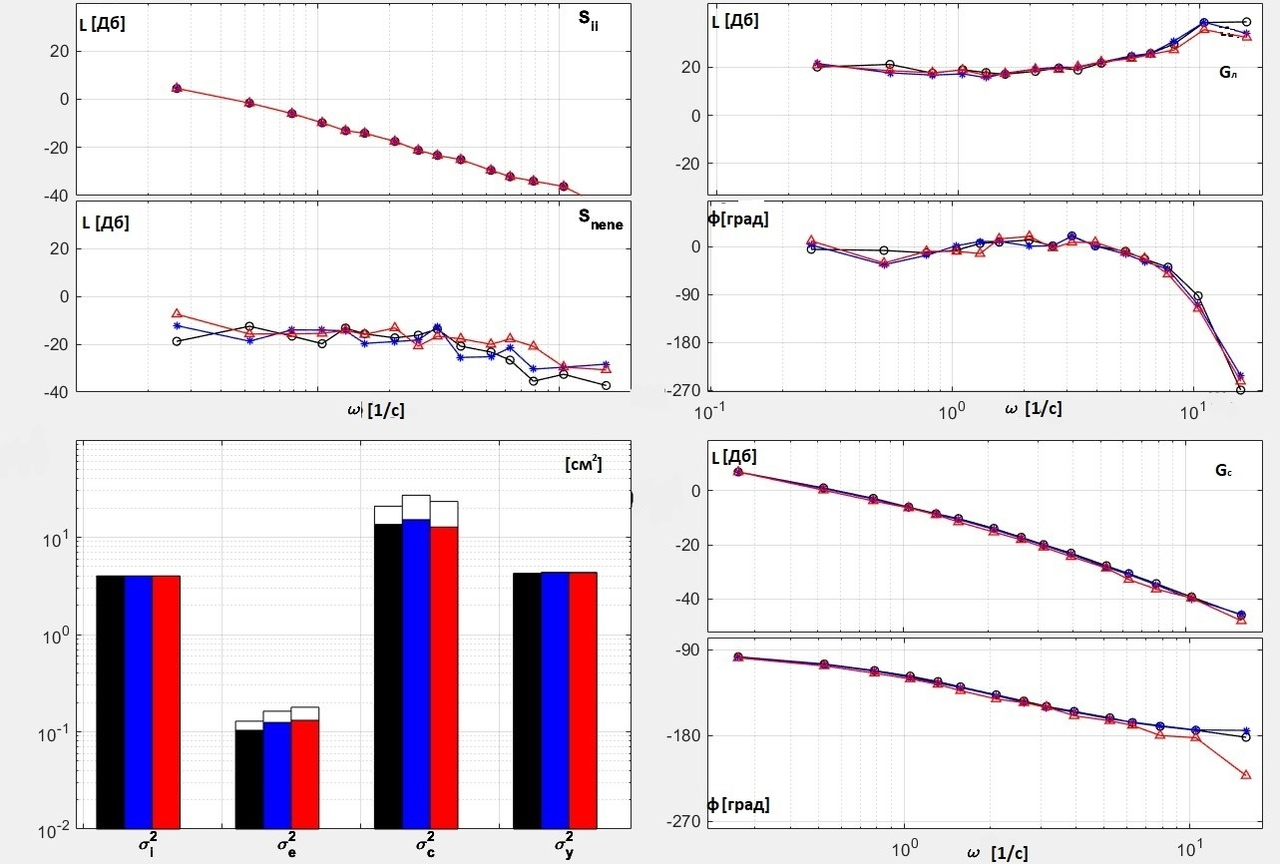
\includegraphics[width=11cm, height = 6cm]{../Оглавление/Part3/figures/Модель без PI.jpg}}
    \end{block}
\end{frame}

% \begin{frame}{Специальная часть}{Результаты исследований}

% \begin{table}[H]
%     \begin{tabular}{|c|c|c|c|}
%         \hline 
%         № э.& $\sigma^2_e,$ см$^2$ & $\sigma^2_c$ см$^2$ & $n_e$ см$^2$ \\ \hline 
%         1& 0.103 & 13.54 & 0.0254\\ \hline
%         2& 0.125 & 15.14  & 0.037 \\ \hline
%         3& 0.131 & 12.74 & 0.047\\ \hline

%     \end{tabular}
% \end{table}
% \end{frame}
 
% \begin{frame}{Специальная часть}{Робастность системы}
% \begin{table}[H]
%     \begin{tabular}{|c|c|c|c|c|}
%         \hline 
%         № э.&Нули & Полюса & $\xi$ & $\omega_c$, 1/c \\ \hline 
%         1& -2 & - & 1.0 &0.5 \\ \hline
%         & -1.9392 & -0.7537  &  & 1.59 $\cdot 10^{-4}$\\ 
%         2& -0.7473 & -0.0161  &1.0 & 1.64 $\cdot 10^{-2}$\\ 
%         & -0.0164 &  0 & &7.47 $\cdot 10^{-1}$\\ 
%         & 0 &   &  &1.94 \\ \hline 
%         & -1.8207 & 0.8255 & &0\\ 
%         3& -0.8033 & -0.0177 & 1.0&1.85 $\cdot 10^{-2}$\\ 
%         & -0.0185 & 0 & &8.03 $\cdot 10^{-1}$ \\ 
%         & 0 &  &  &1.82 \\ \hline
%     \end{tabular}
% \end{table}

% \end{frame}

\begin{frame}{Специальная часть}{Параметры PI-контроллера}
    \begin{block}{Задача PI-контроллера}
        PI-контроллер в теории должен уменьшать сигнал ошибки $e =\delta_\text{э} - \omega_z$, где $k$ - это сигнал входящий в систему.
    \end{block}
    \begin{block}{PI-контроллер}
        $$y(t) = K_p + \frac{1}{p}K_i,$$
        где $K_p = 2$, $K_i = 5$.
        Коэффициенты PI-контроллера были выбраны с условием того, что система должна оставаться устойчива.     
    \end{block}
\end{frame}

\begin{frame}{Специальная часть}{Улучшение робасности с применением PI-контроллера}
    \begin{block}{Схема}
        \center{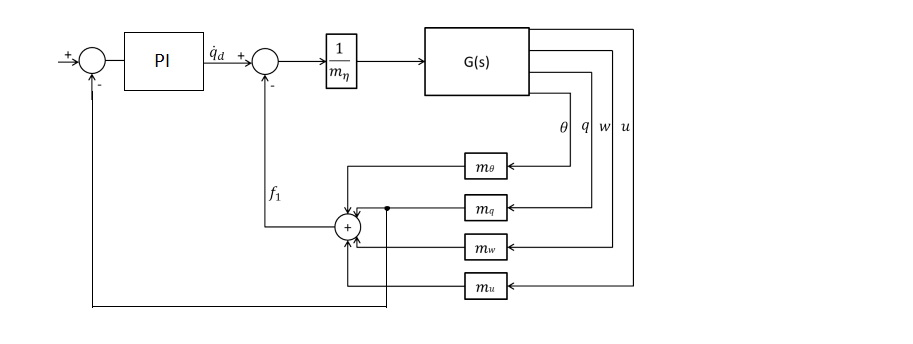
\includegraphics[width=10cm, height = 6cm]{../Оглавление/Part3/figures/Полная схема СПС.png}}
    \end{block}
\end{frame}

\begin{frame}{Специальная часть}{Улучшение робасности с применением PI-контроллера}
    \begin{block}{Результаты экспериментов}
        \center{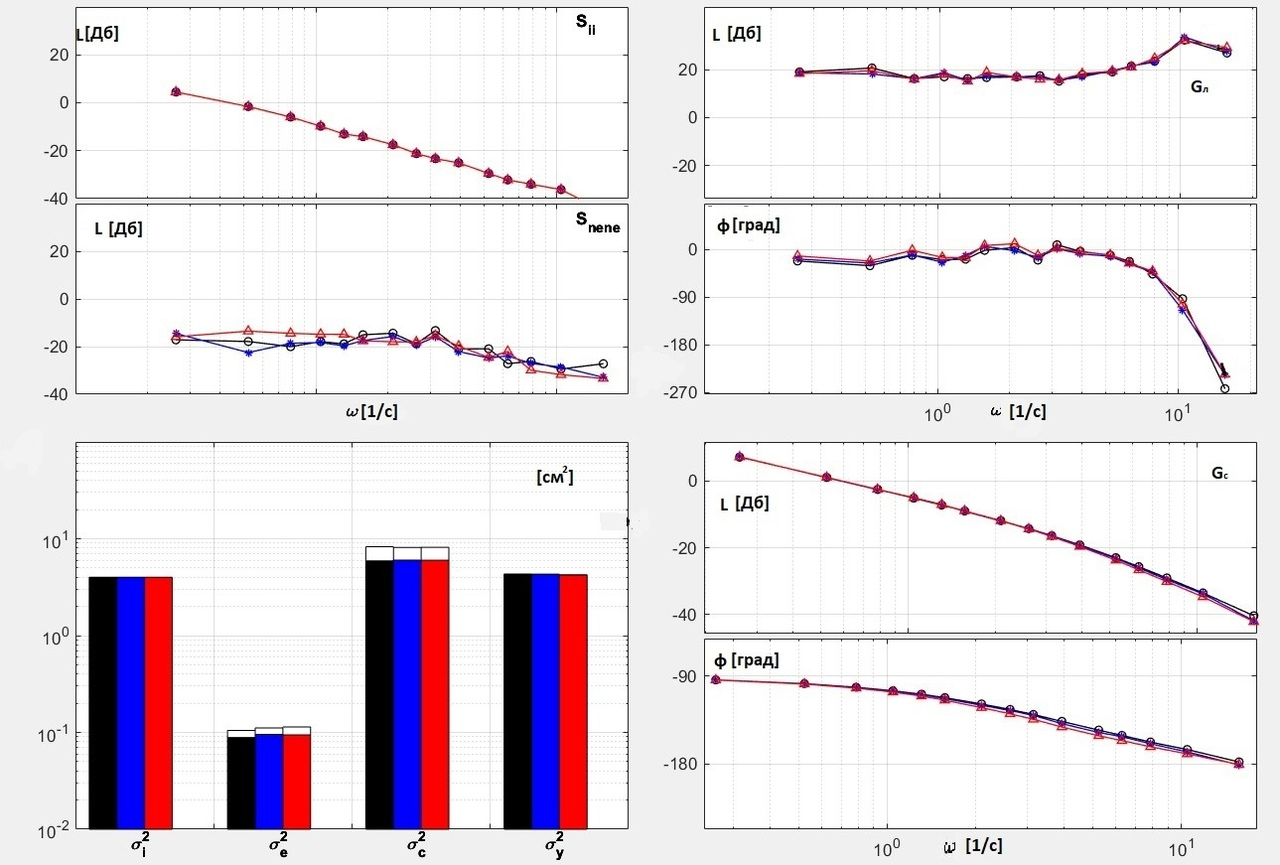
\includegraphics[width=11cm, height = 6cm]{../Оглавление/Part3/figures/Модель с PI.jpg}}
    \end{block}
\end{frame}


% \begin{frame}{Специальная часть}{Результаты исследований}   

% \begin{table}[H]
%     \begin{tabular}{|c|c|c|c|}
%         \hline 
%         № э.& $\sigma^2_e,$ см$^2$ & $\sigma^2_c$ см$^2$ & $n_e$ см$^2$ \\ \hline 
%         1& 0.0886 & 5.913 & 0.01611\\ \hline
%         2& 0.0952 & 6.01  & 0.01591 \\ \hline
%         3& 0.0943 & 6.004 & 0.01712\\ \hline

%     \end{tabular}
% \end{table}
% \end{frame}
 
% \begin{frame}{Специальная часть}{Робастность системы}
% \begin{table}[H]
%     \begin{tabular}{|c|c|c|c|c|}
%         \hline 
%         № э.&Полюса & Нули & $\xi$ & $\omega_c$, 1/c \\ \hline 
%         1& -3.0000 + 1.0000$i$ & -2.5 & 0.95 & 3.16\\ 
%         & -3.0000 - 1.0000$i$ &   &  &  \\ \hline
%         2& -2.8660 + 1.1287$i$ & -0.0161  & 1.0 &  0\\ 
%         & -2.8660 - 1.1287$i$ &  -0.7537 &1.0 & 1.61$\cdot 10^{-2}$\\ 
%         & -0.7547 + 0.0000$i$ &  -2.5000 & 1.0 & 7.51 $\cdot 10^{-2}$\\ 
%         & 0 & 0.0000 & 0.93& 3.08 \\ 
%         & -0.0161 + 0.0000$i$ &  & 0.93 &  \\ \hline 
%         3& -2.5975 + 1.3096$i$ & -0.0177 & 1 & 0\\ 
%         & -2.5975 - 1.3096$i$ & -0.8255 & 1& 1.77 $\cdot 10^{-2}$ \\ 
%         & -0.8292 + 0.0000$i$ & -2.5000 & 1 & 8.29 $\cdot 10^{-1}$\\ 
%         & 0 & 0 & 0.893 & 2.91 \\ 
%         & -0.0177 + 0.0000$i$ &  &  &  \\ \hline 
%     \end{tabular}
% \end{table}
% \end{frame}

% \begin{frame}{Специальная часть}{Переходные процессы}
%     \begin{minipage}[c]{0.45\textwidth}
%         \center{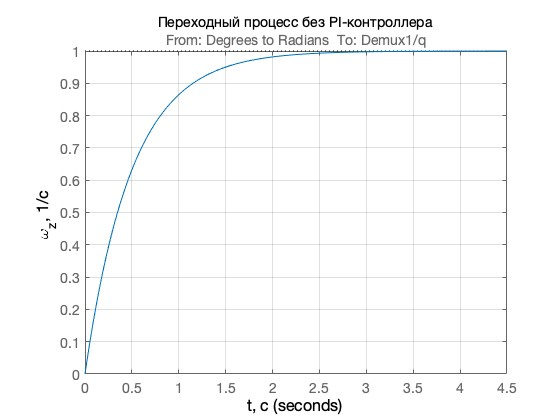
\includegraphics[width=6cm, height = 6cm]{img/withoutPI.jpg}}
%     \end{minipage}
%     \begin{minipage}[c]{0.45\textwidth}
%         \center{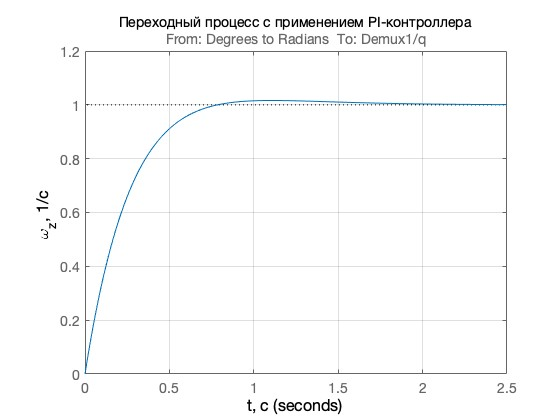
\includegraphics[width=6cm, height = 6cm]{img/withPI.jpg}}
%     \end{minipage}
% \end{frame}
